% ****** Start of file apssamp.tex ******
%
%   This file is part of the APS files in the REVTeX 4.1 distribution.
%   Version 4.1r of REVTeX, August 2010
%
%   Copyright (c) 2009, 2010 The American Physical Society.
%
%   See the REVTeX 4 README file for restrictions and more information.
%
% TeX'ing this file requires that you have AMS-LaTeX 2.0 installed
% as well as the rest of the prerequisites for REVTeX 4.1
%
% See the REVTeX 4 README file
% It also requires running BibTeX. The commands are as follows:
%
%  1)  latex apssamp.tex
%  2)  bibtex apssamp
%  3)  latex apssamp.tex
%  4)  latex apssamp.tex
%
\documentclass[%
 reprint,
%superscriptaddress,
%groupedaddress,
%unsortedaddress,
%runinaddress,
%frontmatterverbose, 
%preprint,
%showpacs,preprintnumbers,
%nofootinbib,
%nobibnotes,
%bibnotes,
 amsmath,amssymb,
 aps,
 article,
%pra,
%prb,
%rmp,
%prstab,
%prstper,
%floatfix,
]{revtex4-1}
 

\usepackage{mathtools}
\usepackage{amsmath}
\usepackage{relsize}
\usepackage{tabto}

\usepackage{graphicx}% Include figure files
\usepackage{dcolumn}% Align table columns on decimal point
\usepackage{bm}% bold math
%\usepackage{hyperref}% add hypertext capabilities
%\usepackage[mathlines]{lineno}% Enable numbering of text and display math
%\linenumbers\relax % Commence numbering lines

%\usepackage[showframe,%Uncomment any one of the following lines to test 
%%scale=0.7, marginratio={1:1, 2:3}, ignoreall,% default settings
%%text={7in,10in},centering,
%%margin=1.5in,
%%total={6.5in,8.75in}, top=1.2in, left=0.9in, includefoot,
%%height=10in,a5paper,hmargin={3cm,0.8in},
%]{geometry}

\begin{document}

%\preprint{APS/123-QED}

\title{Classificatore di generi musicali}% Force line breaks with \\

\author{Matteo Collina}

\affiliation{
 Università degli Studi di Milano\\
}%


\date{\today}% It is always \today, today,
             %  but any date may be explicitly specified

\begin{abstract}
In questo articolo viene presentato un sistema per la classificazione automatica di brani audio in base al genere musicale al quale appartengono. Ogni genere può essere rappresentato come un albero, dal quale si ramificano i suoi sottogeneri, ognuno dei quali possiede un’influenza data da un altro genere musicale o un periodo storico.
\end{abstract}


\maketitle

%\tableofcontents

\section{\label{sec:level1}Introduzione}

In questo articolo viene presentata una comparazione tra vari modelli di classificazione supervisionata. \\\\
L'obiettivo è valutare le performance di ogni modello e identificare quale sia il candidato ideale variando: \textit{la proporzione delle dimensioni degli insiemi di test e training}, \textit{il numero di brani musicali per ogni genere} ed \textit{il numero di generi} totali, mantenendo fisso il numero di feature.\\Per ogni allenamento del modello viene fatto tuning con una serie di parametri, ad esempio il k nel modello kNN, e scelto il valore che massimizza l'accuracy. \\\\
Viene descritto inoltre come vengono memorizzati i dati per la creazione del dataset, come avviene il processo di training del modello e relativo salvataggio sotto forma di file per poter classificare successivamente nuovi brani audio. \\\\
Il lavoro di classificazione viene effettuato su file audio stereo di 30 secondi con frequenza di campionamento a 44100Hz. La scelta è dettata dalla volontà di valutare tutte le informazioni contenute in questo range temporale, senza comprimere il campionamento, scegliendo di rinunciare ad una parte del brano stesso, supponendo che i 30 secondi centrali del brano siano sufficienti. \\\\
Le prove sono state eseguite inizialmente con 5 generi: \textit{Classical, Dance, Jazz, Pop, Rock }, aggiungendone successivamente altri 5:  \textit{Blues, Country, HipHop, Metal, Reggae}.


\section{\label{sec:level1}Stato dell'Arte}

Il problema della classificazione di brani musicali è stato analizzato non solo considerando i file audio ma anche prendendo in causa le immagini del loro spettogramma \cite {spettogrammaClassifier}, oppure unendo l'analisi del brano con quella grafica \cite {spettoAudioClassifier}.


Durante lo svolgimento del progetto sono state utilizzate quattro tecniche di classificazione supervisionata:  \textbf{kNN, SVM, Random Forest e Gradient Boosting} le quali considerano solamente feature ottenute dall'analisi dei file audio. La scelta sulle feature da utilizzare è argomento di discussione come in \cite {featBeat}, in cui viene prestata l'attenzione sulla dipendenza che hanno le feature con il genere. \\

Altra panoramica presente per la classificazione di un brano musicale si basa sullo studio del linguaggio dei testi condotta in \cite {lyrics}, la quale propone un approccio di Information Retrieval basato primariamente sul NLP.\\

\textbf{Panoramica sui metodi di classificazione utilizzati}:\\

\paragraph{kNN}
Un oggetto, rappresentato attraverso vettori di posizione in uno spazio multidimensionale, è classificato in base alla maggioranza dei voti dei suoi k vicini, i quali devono essere sempre dispari per assicurarsi che venga presa una decisione. Come misura di distanza viene utilizzata la \textit{distanza Euclidea} tra i vettori. Nel sistema viene testata questa serie di parametri: \textit{1,3,5,7,9,11,13,15}. 

\paragraph{SVM}
Si basa sul concetto di piani decisionali che definiscono dei confini. Un piano decisionale (iperpiano) è una porzione di superficie che separa insiemi di punti appartenenti a classi diverse. Se i punti non fossero linearmente separabili potremmo alterare lo spazio aggiungendo una dimensione tramite una tecnica chiamata  \textbf{Kernel Trick}. Nel sistema vengono utilizzati i seguenti parametri di valutazione: \textit{0.001, 0.01, 0.5, 1.0, 5.0, 10.0, 20.0} che corrispondono alla dimensione dell'iperpiano (per valori elevati di C, l'ottimizzazione sceglierà un iperpiano a margine più piccolo).

\paragraph{Random Forest}

E' un algoritmo \textit{ensemble}, ovvero che combina più di un algoritmo per classificare oggetti (es, SVM, Naive Bayes, Decision Trees) e  \textit{bagging}, per cui la costruzione dei predittori è fatta in maniera indipendente.
L'idea generale è che sia selezionata una combinazione di modelli di apprendimento che aumenti il risultato complessivo. I parametri per il tuning indicano il numero di trees utilizzati per la classificazione.

\paragraph{Gradient Boosting}
Anche questo metodo è \textit{ensemble} ma, a differenza del Random Forest, creare un pool di predittori a cascata (\textit{boosting}), in cui ogni output è l'input del modello seguente. Esso presenta molti più parametri per fare tuning, rendendolo più incline all'overfitting rispetto al Random Forest ma, trovata la giusta combinazione di parametri, restituisce valori migliori del primo. I parametri utilizzati nella classificazione indicano il numero di boosting stages.


\section{\label{sec:level1}Implementazione}

Inizialmente viene effettuata una chiamata REST  \cite {musixmatch} al servizio \textbf{MusixMatch} per recuperare tutti i generi musicali presenti nel database, i quali vengono aggiunti ad una collezione locale di MongoDb. Prima dell'effettivo salvataggio, si itera sull'array di json restituito dalla chiamata e si effettua un mapping tra il genere corrente e la classe del modello di training, il quale ci servirà in fase di valutazione di un singolo brano ottenuto dalle API di MusixMatch.\\
Gli id di questi ultimi vengono utilizzati successivamente per recuperare le informazioni delle canzoni catalogate con quel determinato genere, creando la \textit{Ground truth}, salvate poi in un'altra collezione del db.\\\\
Si itera inoltre sugli elementi nella collezione, contenente le informazioni delle canzoni e, tramite la libreria Youtube-Dl \cite {ytdl}, si scarica il file audio in locale. Viene effettuata un'elaborazione del file, convertendolo nel formato WAV, e selezionando i 30 secondi centrali del brano per ottimizzare lo storage ed eliminare la parte iniziale e finale che, nella maggior parte dei casi,non è musicale.\\\\
\textbf{pyAudioAnalysis} \cite {pyAudioAnalysis} è la libreria utilizzata per le operazioni di feature extraction e classificazione supervisionata di segnali audio.
\paragraph{Feature Extraction} Sono gestite 70 features in totale \cite {feattype}, tra le quali la \textit{Beat Extraction}, la quale fornisce un metodo per la stima della frequenza dei battiti al minuto (BPM) di un segnale musicale che sarà rilevante per questo sistema. Viene creata una matrice contenente più matrici le quali rappresentano i vari generi musicali. Ognuna di esse avrà più feature vector al suo interno, ognuno rappresentante un brano musicale per quel determinato genere.

\paragraph{Normalizzazione delle feature} \cite {norm}
Viene rimosso il livello del genere nella matrice delle feature, e calcolata la media aritmetica per ogni i-esima feature di ogni vettore. Analogamente viene calcolata la deviazione standard ed infine viene eseguita la seguente operazione di normalizzazione: 

$X = Matrice$ $delle$ $features$
\larger[1.5]
\begin{align*}
z_{ij} = \frac{ x_{ij} - \mu_{j} } {\sigma_{j} }
\end{align*}
\relsize{-1.5}

Nella \textbf{z-standard normalization} ogni valore rappresenta il gap di quanto si discosta dalla media, prendendo come unità di misura la deviazione standard. 
Nel caso in cui si trasformano i punteggi osservati in punteggi z si ottiene una particolare curva che ha media uguale a 0 e varianza uguale a 1 ed è chiamata \textit{distribuzione normale standardizzata}.

\paragraph{Scelta miglior parametro}
Esegue una procedura di convalida incrociata per selezionare il parametro di classificazione ottimale per il problema in esame (es. Il valore di k per il classificatore kNN). Durante l'iterazione dei parametri vengono eseguite le seguenti operazioni:

\subparagraph{Creazione matrice di Training e Test}
Viene suddivisa la matrice delle feature in due, una per il training ed una per il test per mezzo di un parametro che indica le proporzioni da mantenere tra le loro dimensioni.

\subparagraph{Creazione modello di training}
Si crea il classificatore passando la matrice temporanea di training, ottenuta nel punto precedente. Per ogni matrice di test di ogni classe, si valuta ogni feature vector a quale classe è più affine ed ogni voto positivo comporta un incremento di 1 nella relativa locazione della matrice contenente i risultati, riferita a quel determinato genere.

\subparagraph{Calcolo Valutazione}
Completata l'iterazione sul numero di esperimenti totali per quel determinato parametro, vengono calcolate: precision, recall, f1-misure e accuracy.

\begin{align*}
Recall:
\frac{ True\ Positive } { True\ Positive + False\ Negative }
\\\\
Precision:
\frac{ True\ Positive } { True\ Positive + False\ Positive }
\\\\
f1:
\frac{ 2* Precion * Recall } {Precision + Recall}
\\\\
Accuracy:
\frac{ TP + TN } { TP\ + TN\ + FP\ + FN }
\end{align*}


Una volta testati tutti i parametri per quel modello, si può scegliere se restituire il parametro che ha portato una miglior accuracy o la migliore media di f1 dei generi.
\\
\paragraph{Stampa Confusion Matrix}
Viene stampata la confusion matrix e salvati i valori in un file \textit{csv}, moltiplicandoli per una costante 100 per una miglior lettura. Vengono salvati inoltre tutti i risultati ottenuti per ogni parametro del modello di training valutato.
\\
\paragraph{Salvataggio modello}
Viene salvato su file il modello di training per rendere possibile la valutazione di un brano successivamente.



\section{\label{sec:level1}Risultati}
Le macro-categorie di test effettuati sono state:
\paragraph{10 generi musicali, ognuno contenente 100 file audio, con rapporto Training/Test a ~ 90\% e 70\%}:\\

\begin{figure} [h!]
  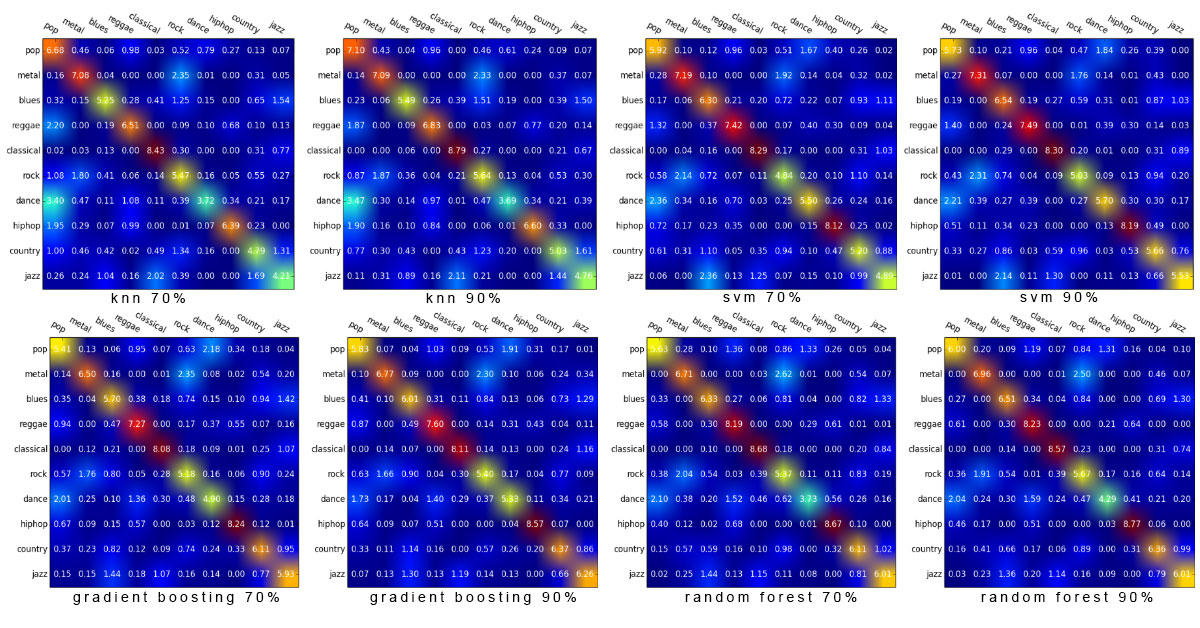
\includegraphics[width=\linewidth]{images/Results-100tracksPerGenre-10genres.jpg}
  \caption{Risultati per 10 generi musicali, ognuno avente 100 brani audio}
  \label{fig:r_10_100}
\end{figure}


L'algoritmo \textbf{kNN} non riesce a distinguere le differenze del genere \textit{Dance} da quello \textit{Pop} fornendo probabilità attese molto simili. Questa distinzione non risulta avvenire se si prende in esame il genere \textit{Pop}, il quale non risulta essere affine alla classe \textit{Dance} seppure i due generi siano influenzati l'uno dall'altro. Esso riesce a mantenere una buona distinzione tra i generi "padre" dai loro discendenti, si può notare tra \textit{Jazz} e \textit{Classical}, nel quale il primo sia evidentemente affine al secondo, a distinzione del contrario in cui il genere Classical  non presenta il ritmo posseduto dal \textit{Jazz}, fornendo una probabilità inferiore. Si può notare inoltre un' inaspettata correlazione tra il genere \textit{Reggae} e quello \textit{Pop}. 

Il classificatore \textbf{SVM} a differenza del primo riesce a distinguere in modo migliore le differenze tra \textit{Pop} e \textit{Dance}, seppure la loro influenza. Si può notare come il valore di \textit{Dance} della diagonale sia pari al 57\%, a differenza del 37\% restituito da kNN con un incremento del 20\%. Le probabilità attese inaspettate nel kNN vengono annullate, proponendo valori bassi rappresentativi della realtà. Inoltre il genere \textit{Jazz} risulta essere più vicino al genere \textit{Blues} rispetto alla musica classica, in contrapposizione ai risultati del kNN.\\

Gli algoritmi \textbf{Gradient Boosting} e \textbf{Random Forest} presentano risultati molto simili tra di loro. Si può notare in entrambi un'affinità considerevole del genere \textit{Dance} con \textit{Reggae}, soprattutto nel Random Forest, il quale presenta un valore ridotto nella diagonale, migliorando visibilmente con un insieme di training pari al 90\%. In quest'ultimo si presenta però un miglioramento della riga riferita alla classe \textit{Reggae}, la quale non fornisce indicazioni di influenze con gli altri generi.

Considerando la suddivisione al 90\% degli insiemi di test e training, la miglior valutazione proviene dal Random Forest (accuracy: 67.37, f1 misure: 67.03), mentre la peggiore dal kNN (Accuracy: 60.9, f1 misure: 58.55)
\\
\paragraph{10 generi musicali, ognuno contenente 170 file audio, con rapporto Training/Test a ~ 90\% e 70\%}:

\begin{figure} [h!]
  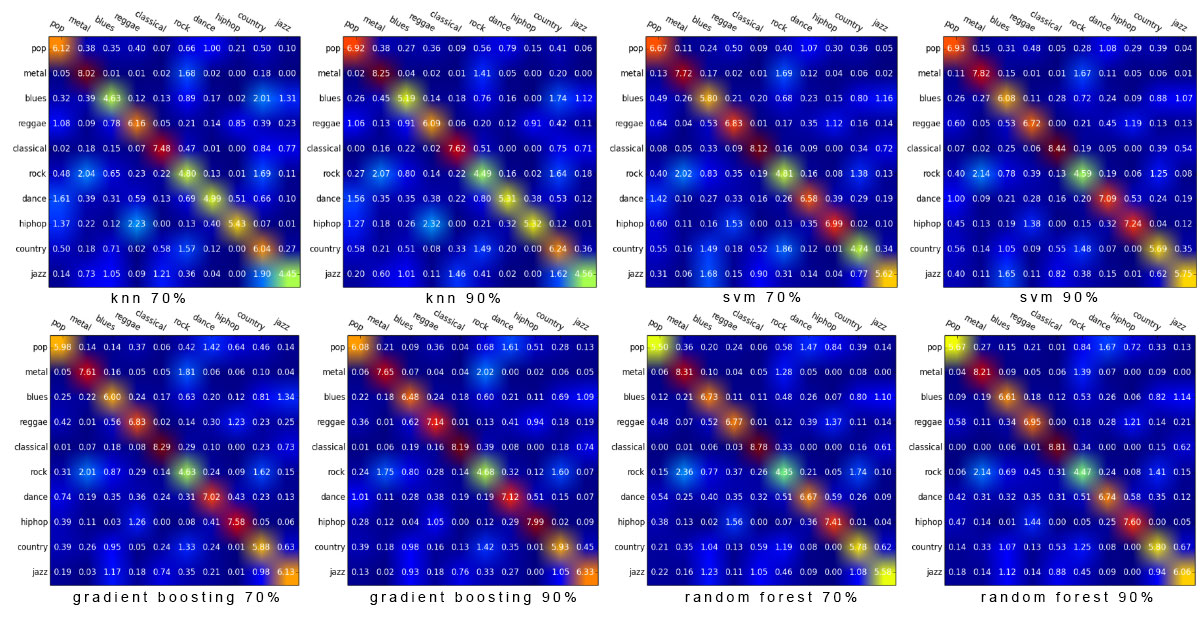
\includegraphics[width=\linewidth]{images/Results-170tracksPerGenre-10genres.jpg}
  \caption{Risultati per 10 generi musicali, ognuno avente 170 brani audio}
  \label{fig:r_10_170}
\end{figure}

Rispetto ai risultati ottenuti nel primo test, notiamo come l'affinità del genere \textit{Dance} con il genere \textit{Pop} si riduca notevolmente con l'algoritmo Random Forest, mentre viene correttamente ridimensionata nell'SVM. Con l'aumento del numero di brani, il kNN si conferma l'algoritmo con i valori nella diagonale più bassi degli altri presi in analisi assumendo considerevoli influenze tra i generi.\\
Al crescere del numero di brani la miglior valutazione proviene dal Gradient Boosting (accuracy: 67.58, f1 misure: 67.64), mentre la peggiore proviene sempre dal kNN (Accuracy: 58.09, f1 misure: 58.20).\\
Come ultimo tentativo è stato applicato il Kernel Trick (\textit{Gaussian Kernel}) all'SVM provocando un aumento rilevante dell'accuracy (70.59) e della f1 (70.48). 

\begin{figure} [h!]
  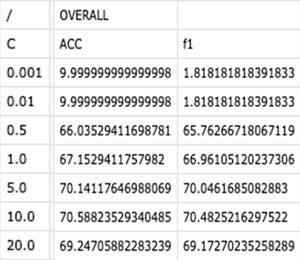
\includegraphics[width=50mm,scale=0.5]{images/params.jpg}
  \caption{Accuracy e f1 risultanti dal SVM, Gaussian Kernel}
  \label{fig:r_svm_gaussia_paramsl}
\end{figure}


\paragraph{5 generi musicali, ognuno contenente 100 file audio, con rapporto Training/Test a ~ 90\% e 70\%}:

\begin{figure} [h!]
  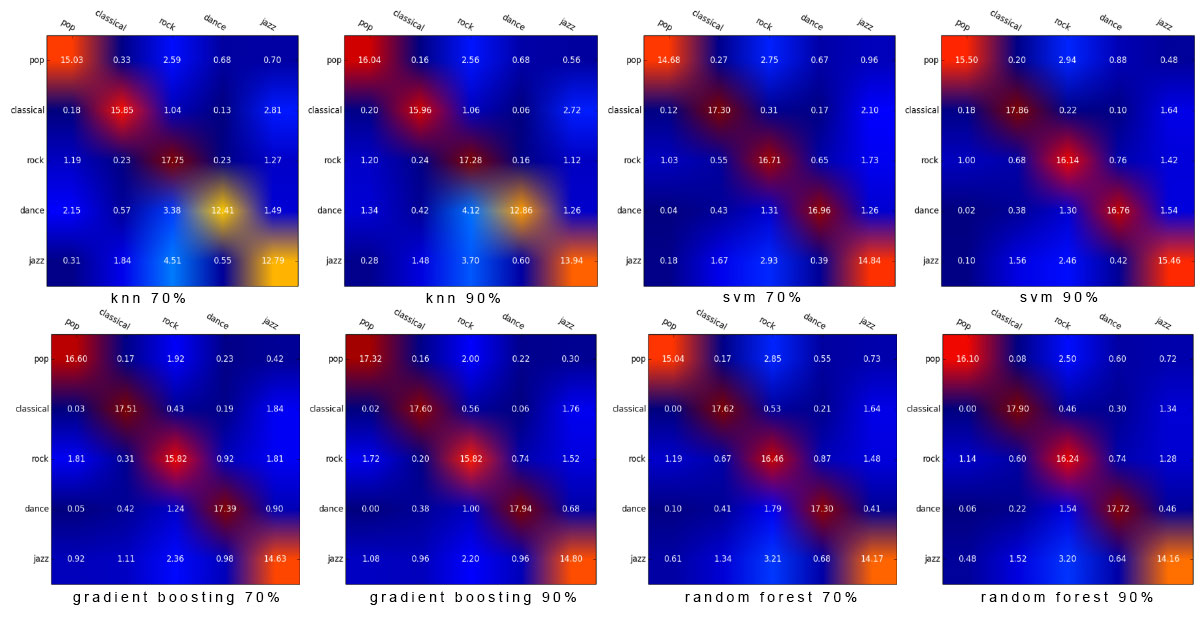
\includegraphics[width=\linewidth]{images/Results-100tracksPerGenre-5genres.jpg}
  \caption{Risultati per 5 generi musicali, ognuno avente 100 brani audio}
  \label{fig:r_5_100}
\end{figure}

Dimezzando il numero di classi si nota come l'unico algoritmo in grado di considerare correlazioni tra i generi sia il kNN. Infatti risulta essere l'unico a segnalare una relazione tra Pop e Dance, che viene azzerata negli altri tre modelli. 


\section{\label{sec:level1}Conclusioni}
In conclusione, all'aumentare del numero di brani per genere, il miglior algoritmo da adottare per la classificazione risulta essere l'\textbf{SVM} con una suddivisione del training set pari al 90\% e con l'applicazione di una funzione kernel (nel nostro caso è stata valutata la Gaussian Kernel). Oltre a mantenere la miglior accuracy e f1 misure, restituisce risultati ragionevoli per i valori non disposti sulla diagonale. \\
Con un numero ridotto di classi (\textless= 5) si può pensare di adottare il \textbf{kNN}, unico che riesce ad intuire relazioni tra di esse. Esso presenta un peggioramento all'aumentare del numero di generi, poiché i documenti nello spazio tenderanno ad essere sempre più vicini e compatti, producendo interferenza tra di essi.\\ 
Il Gradient Boosting risulta essere il modello che prende decisioni più sicure, ovvero il genere risultante avrà una probabilità molto più alta rispetto alle altre, a differenza del  \textbf{Random Forest} il quale mantiene proporzioni simili per i primi risultati. Questo avviene poichè i modelli \textit{boosting} aggregano in modo sequenziale i predittori, pertanto ognuno di essi potrà tener conto dell'errore del modello precedente. Entrambi vengono utilizzati anche per fare regressione, pertanto risultano essere tool più predittivi che descrittivi.\\\\

In conclusione, i risultati non sono ottimali, soprattutto di generi con molte influenze. Il genere pop non viene quasi mai scelto dal classificatore perchè risulta difficile descriverlo con 170 brani ed inoltre varia di anno in anno, a differenza dei generi che rimangono invariati, tra i quali: metal, rock, country, jazz e blues. Pertanto per la musica dance e pop si dovrebbero creare più categorie in base ai decenni ('80,'90,'00), mentre per il genere hiphop distinguerlo dal genere trap, il quale si è inserito nella scena pop di molti paesi europei. Infine risulta evidente quanto non sia sufficiente creare categorie per i macro generi, ma sia necessario sottoporli ad un ulteriore \textit{suddivisione in base al momento storico}.


\begin{thebibliography}{1}

  \bibitem{spettogrammaClassifier} Julien Despois {\em Finding the genre of a song with Deep Learning}  2016.
 
  \bibitem{spettoAudioClassifier} Hareesh Bahuleyan {\em Music Genre Classification using Machine Learning Techniques} 2018.
 
  \bibitem{featBeat} Juan Jose Burred, Alexander Lerch {\em  A HIERARCHICAL APPROACH TO
AUTOMATIC MUSICAL GENRE CLASSIFICATION} 2003.

  \bibitem{lyrics}  Jose P. G. Mahedero, Alvaro Martinez, Pedro Cano, Markus Koppenberger, and
Fabien Gouyon.  {\em Natural language processing of lyrics. In MULTIMEDIA ’05:
Proceedings of the 13th annual ACM international conference on Multimedia, pages
475–478}, New York, NY, USA, 2005. ACM Press.

\bibitem{musixmatch} https://developer.musixmatch.com/documentation/api-methods
\bibitem{ytdl} https://rg3.github.io/youtube-dl/

\bibitem{pyAudioAnalysis} Theodoros Giannakopoulos {\em https://github.com/tyiannak/pyAudioAnalysis} 2015.

\bibitem{feattype} https://github.com/tyiannak/pyAudioAnalysis/wiki/3.-Feature-Extraction

\bibitem{norm} https://pellerey.unisal.it/052006.pdf {\em I punteggi zeta e la distribuzione normale}


  \end{thebibliography}


\end{document}


 

%
% ****** End of file apssamp.tex ******
